\documentclass[11pt]{article} 
\usepackage[english]{babel}
\usepackage[utf8]{inputenc}
\usepackage[margin=0.5in]{geometry}
\usepackage{amsmath}
\usepackage{amsthm}
\usepackage{amsfonts}
\usepackage{amssymb}
\usepackage[usenames,dvipsnames]{xcolor}
\usepackage{graphicx}
\usepackage[siunitx]{circuitikz}
\usepackage{tikz}
\usepackage[colorinlistoftodos, color=orange!50]{todonotes}
\usepackage{hyperref}
\usepackage[numbers, square]{natbib}
\usepackage{fancybox}
\usepackage{epsfig}
\usepackage{soul}
\usepackage[framemethod=tikz]{mdframed}
\usepackage[shortlabels]{enumitem}
\usepackage[version=4]{mhchem}
\usepackage{multicol}

\usepackage{mathtools}
\usepackage{comment}
\usepackage{enumitem}
\usepackage[utf8]{inputenc}
\usepackage[linesnumbered,ruled,vlined]{algorithm2e}
\usepackage{listings}
\usepackage{color}
\usepackage[numbers]{natbib}
\usepackage{subfiles}
\usepackage{tkz-berge}


\newtheorem{prop}{Proposition}[section]
\newtheorem{thm}{Theorem}[section]
\newtheorem{lemma}{Lemma}[section]
\newtheorem{cor}{Corollary}[prop]

\theoremstyle{definition}
\newtheorem{definition}{Definition}

\theoremstyle{definition}
\newtheorem{required}{Problem}
\newtheorem*{requiredHC}{Problem HC}

\theoremstyle{definition}
\newtheorem{ex}{Example}


\setlength{\marginparwidth}{3.4cm}
%#########################################################

%To use symbols for footnotes
\renewcommand*{\thefootnote}{\fnsymbol{footnote}}
%To change footnotes back to numbers uncomment the following line
%\renewcommand*{\thefootnote}{\arabic{footnote}}

% Enable this command to adjust line spacing for inline math equations.
% \everymath{\displaystyle}

% _______ _____ _______ _      ______ 
%|__   __|_   _|__   __| |    |  ____|
%   | |    | |    | |  | |    | |__   
%   | |    | |    | |  | |    |  __|  
%   | |   _| |_   | |  | |____| |____ 
%   |_|  |_____|  |_|  |______|______|
%%%%%%%%%%%%%%%%%%%%%%%%%%%%%%%%%%%%%%%

\newcommand{\standard}{26}

\title{
\normalfont \normalsize 
\textsc{CSCI 3104 Fall 2022 \\ 
Instructors: Prof. Grochow and Chandra Kanth Nagesh} \\
[10pt] 
\rule{\linewidth}{0.5pt} \\[6pt] 
\huge Midterm S\standard \\
\rule{\linewidth}{2pt}  \\[10pt]
}
%\author{Your Name}
\date{}

\begin{document}
\definecolor {processblue}{cmyk}{0.96,0,0,0}
\definecolor{processred}{rgb}{200, 0, 0}
\definecolor{processgreen}{rgb}{0, 255, 0}
\DeclareGraphicsExtensions{.png}
\DeclareGraphicsExtensions{.gif}
\DeclareGraphicsExtensions{.jpg}

\maketitle


%%%%%%%%%%%%%%%%%%%%%%%%%
%%%%%%%%%%%%%%%%%%%%%%%%%%
%%%%%%%%%%FILL IN YOUR NAME%%%%%%%
%%%%%%%%%%AND STUDENT ID%%%%%%%%
%%%%%%%%%%%%%%%%%%%%%%%%%%
\noindent
Due Date \dotfill Saturday Nov 19, 2022 4pm MT \\
Name \dotfill \textbf{Tyler Huynh} \\
Student ID \dotfill \textbf{109603994} \\
Quiz Code (enter in Canvas to get access to the LaTeX template) \dotfill \textbf{ul0UsWwUAs}


\tableofcontents

\section*{Instructions}
\addcontentsline{toc}{section}{Instructions}
 \begin{itemize}
	\item You may either type your work using this template, or you may handwrite your work and embed it as an image in this template. \textbf{If you choose to handwrite your work, the image must be legible, and oriented so that we do not have to rotate our screens to grade your work.} We have included some helpful LaTeX commands for including and rotating images commented out near the end of the LaTeX template.
	\item You should submit your work through the \textbf{class Gradescope page} only. Please submit one PDF file, compiled using this \LaTeX \ template.
	\item You may not need a full page for your solutions; pagebreaks are there to help Gradescope automatically find where each problem is. Even if you do not attempt every problem, please submit this document with no fewer pages than the blank template (or Gradescope has issues with it).

	\item You \textbf{may not collaborate with other students}. \textbf{Copying from any source is an Honor Code violation. Furthermore, all submissions must be in your own words and reflect your understanding of the material.} If there is any confusion about this policy, it is your responsibility to clarify before the due date. 

	\item Posting to \textbf{any} service including, but not limited to Chegg, Discord, Reddit, StackExchange, etc., for help on an assignment is a violation of the Honor Code.

	\item You \textbf{must} virtually sign the \hyperlink{HonorCode}{Honor Code}. Failure to do so will result in your assignment not being graded.
\end{itemize}


\newpage
\section*{Honor Code (Make Sure to Virtually Sign)} \label{HonorCode}
\addcontentsline{toc}{section}{Honor Code (Make Sure to Virtually Sign)}
\hypertarget{HonorCode}{}

\begin{requiredHC}
\begin{itemize}
\item My submission is in my own words and reflects my understanding of the material.
\item Any collaborations and external sources have been clearly cited in this document.
\item I have not posted to external services including, but not limited to Chegg, Reddit, StackExchange, etc.
\item I have neither copied nor provided others solutions they can copy.
\end{itemize}

%\noindent In the specified region below, clearly indicate that you have upheld the Honor Code. Then type your name. 
\end{requiredHC}

\begin{proof}[I agree to the above, Tyler Huynh.]
%% Typing "I agree to the above," followed by your name is sufficient.
\end{proof}


\newpage
\setcounter{section}{\standard-1}
\section{Standard \standard: Hash Tables}

\setcounter{required}{\standard-1}
\begin{required} 
Consider a hash table designed to store integers, using the hash function $h(k)=k~mod~5$ for all keys $k$ for a table of size 5. (Resolve collisions by chaining with a linked list.) You have three scenarios: 
\begin{itemize}
\item Scenario 1: keys are randomly drawn from integers that are divisible by 5.

\item Scenario 2: keys are randomly drawn from integers of the form $5m+1$ where $m$ is an integer.

\item Scenario 3: keys are randomly drawn from \emph{all} integers
\end{itemize}


\noindent \\ Do the following.
\begin{enumerate}[label=(\alph*)]
\item For which scenario does the hash function $h(k)$ perform better? Please  {\bf explain/justify} your answer.


\begin{proof}[Answer]
Scenario 3, will perform better because for both scenario one and scenario two these two scenarios will always hash the keys to the same bucket such that, scenario 1 will always hash it to bucket 0 creating a collision and scenario 2 will always hash it to bucket 1 also creating a collision. Scenario 3 since we are drawing from all integers the likelihood of a collision happening is less than both scenario 1 and 2 because we can hash to buckets from 0 to 4.
\end{proof}

\newpage

\item In each of the three applications, does the hash function $h(k)$ satisfy the uniform hashing property? Please {\bf explain/justify} your answer.

\begin{proof}[Answer]
\textbf{Scenario 1:} Would not satisfy the uniform hashing property because it would satisfy the second condition where two keys $k$ are independent, but it will fail the first one where the probability of hashing any key into any index should be $\frac{1}{5}$ however it is not as the probability of hashing the key into bucket 0 will always be 1, because the key will always be divisible by 5. The probability of hashing any other key into another would be 0. Thus it does not satisfy the uniform hashing property. \\

\textbf{Scenario 2:} Would not satisfy the uniform hashing property because it would satisfy the second condition where two keys $k$ are independent, but it will fail the first one where the probability of hashing any key into any index should be $\frac{1}{5}$ however it is not as the probability of hashing the key into bucket 1 will always be 1, because the key will always have a remainder of 1 by the definition of the scenario and h(k). The probability of hashing any other key into another would be 0. Thus it does not satisfy the uniform hashing property. \\ 

\textbf{Scenario 3:} This scenario would satisfy the uniform hashing property because the second condition will be satisfied such that two keys within h(k) are independent from one another. This scenario would also satisfy the first condition because we are drawing the keys randomly from all integers, the probability of hashing the key into any of the 5 buckets will be $\frac{1}{5}$, where 5 represents $m$ or the number of buckets. 
\end{proof}

\newpage

\item Suppose you have $n$ keys in total for each application. What is the resulting load factor for each application?

\begin{proof}[Answer]
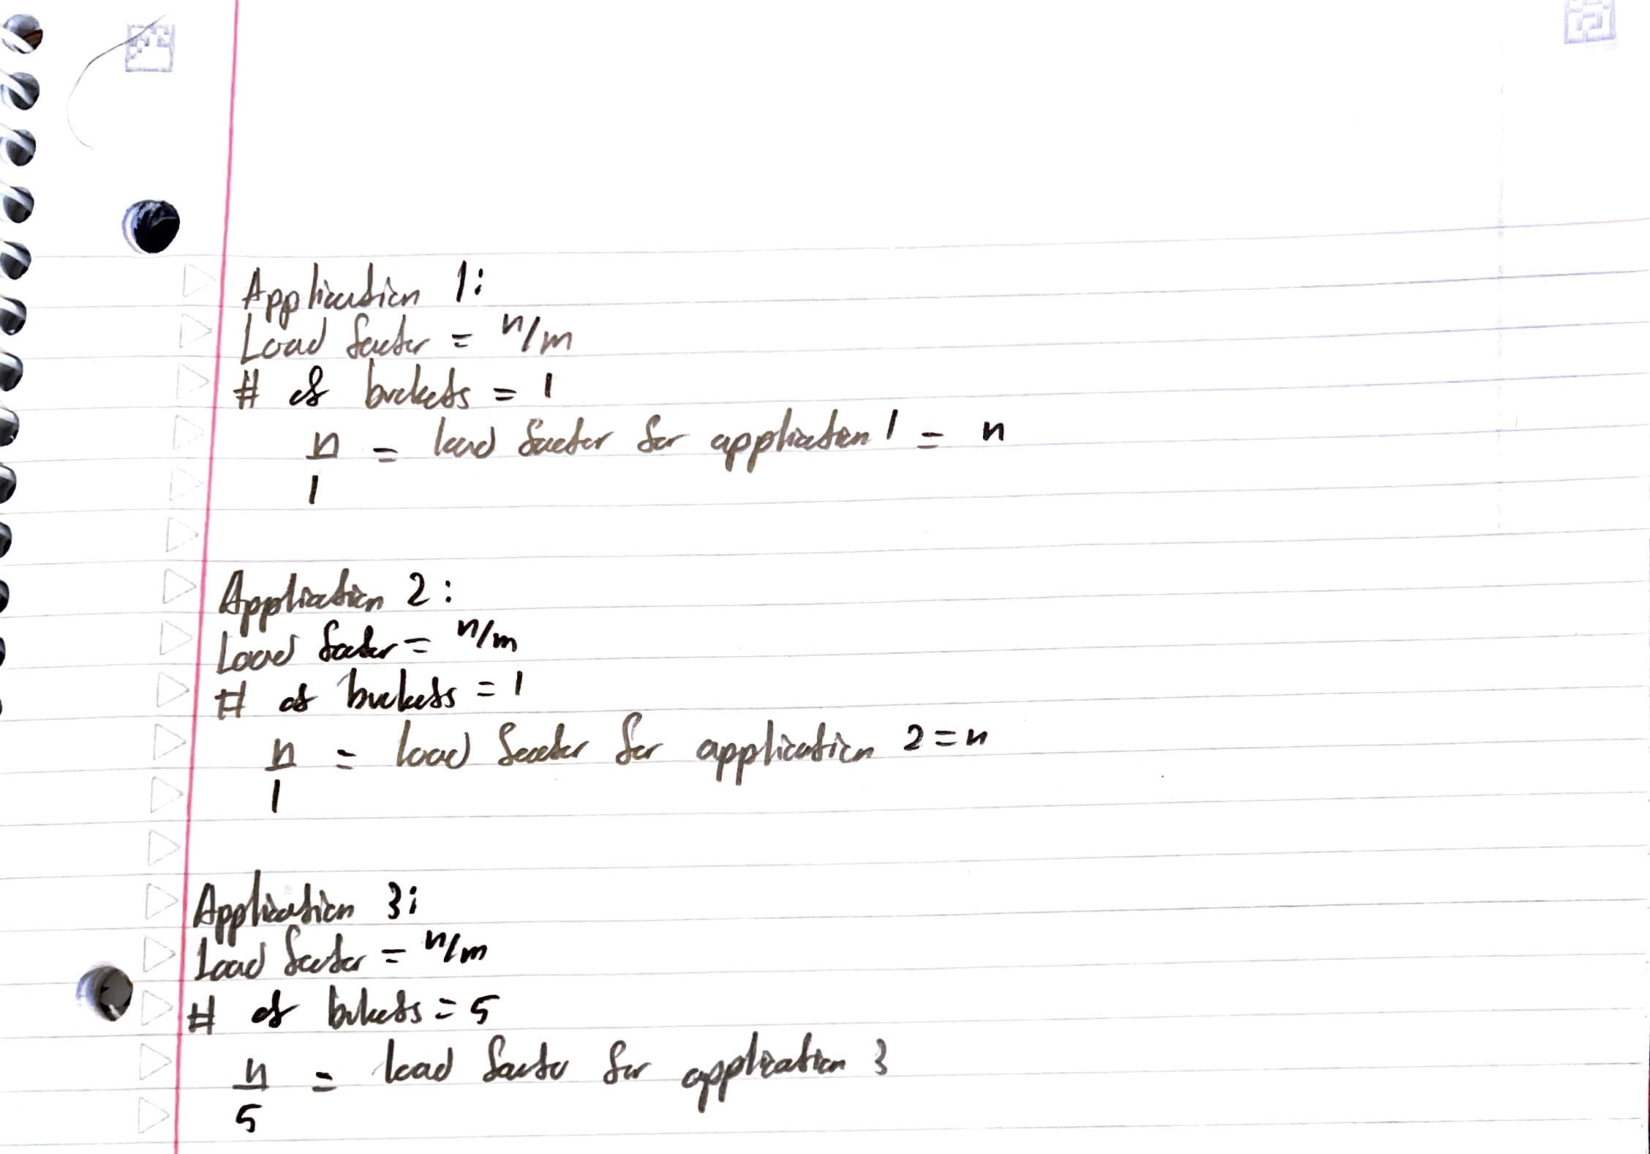
\includegraphics[width=0.9\textwidth]{M2S26Q3.pdf}

\end{proof}

\newpage

\item Suppose you have $n$ keys in total for each application. What are the time complexities of the dictionary operations: add, delete, and find, respectively?

\begin{proof}[Answer]
For all three applications the time complexity of the dictionary: adding will always be $\Theta(1)$ regardless if it  satisfies the uniform hashing property or not because the hash function will always run in constant time when adding something to the hash table. 
\begin{itemize}
\item \textbf{Application 1:} \\
For this application because it does not satisfy the uniform hashing property the runtime for both delete and find using chaining to solve collisions in a linked list, respectively will be $\Theta(n)$. \\
\item \textbf{Application 2:} \\
For this application because it does not satisfy the uniform hashing property the runtime for both delete and find using chaining to solve collisions in a linked list, respectively will be $\Theta(n)$. \\
\item \textbf{Application 3:} \\
For this application since it does satisfy the uniform hashing property per it being able to hash values across all 5 buckets uniformly the runtime for delete and find will be $\Theta(1 + \alpha)$, where $\alpha$ represents our load factor, our load factor by $\frac{n}{m}$ where $n$ represents our keys and $m$ represents the number of buckets we have which 5, such that: 
\begin{center}
Deletion: $\Theta(1 + \frac{n}{5})$ \\
Find: $\Theta(1 + \frac{n}{5})$ \\
\end{center}

\end{itemize}
\end{proof}

\end{enumerate}
\end{required}


% Either type your answer in above, or uncomment the \includegraphics command
% and use it to insert an approprate image. Try experimenting with the scale 
% 0.9 the width option to resize your image if necessary.

%\includegraphics[width=0.9\textwidth]{solution.jpg}


%%%%%%%%%%%%%%%%%%%%%%%%%%%%%%%%%%%%%%%%%%%%%%%%%%
\end{document} % NOTHING AFTER THIS LINE IS PART OF THE DOCUMENT



